\subsection{個人的選好の自由と多数決決定法}
我々はなにか決め事をしようとすると多数決を使います.アローの不可能性定理より,当然多数決もアローの4条件を満たしません.では,どの条件は満たして,どの条件は満たさないのでしょうか.

まずは多数決決定法の定義をしましょう.
\begin{dfn}[多数決決定法]
    任意の2選択肢$x,y$に対して,社会的選好を
    \begin{equation*}
        x \succeq y \leftrightarrow (N(x > y) \ge N(y > x)) \hspace{1cm} (Nはその選好をする個人の数)
    \end{equation*}
    と決定する方法を多数決決定法といいます.
\end{dfn}

これは,我々が日常的に多数決と呼んでいるものとは少し違うことに気をつけてください.一人一票で選択肢に投票する方式はここでは単記投票方式と呼んで区別することにします.多数決決定法は,すべての選択肢のペアに対して二択の単記投票をし,それを社会的選好としてまとめる方法です.

まず,多数決決定法が個人的選好の自由を満たさないことはすでに述べました.昼ご飯の例のような循環が起こりえます.

社会の決定性は満たされます.n人の個人で賛成・反対のどちらかに投票してn人が賛成,0人が反対なら,多数決でも当然結果は賛成になります.

無関係選択肢からの独立性も満たされます.多数決決定法の式を見ると,ある2つの選択肢$x,y$の間での社会的選好は,$x>y$とする人数と$x<y$とする人数にのみ依存します.

非独裁制も満たされます.なぜならば多数決には匿名性があり権力者たれど1人1票なので,1人だけが賛成した時,他に1人でも反対の人がいれば当然結果は賛成にはなりえず,社会的選好に対する独裁者は存在できません.

こう見ると,多数決は個人的選好の自由以外はすべて満たしています.では,今度は,個人的選好の自由をどの程度制限すれば多数決はこの条件を満たすのかについて考えてみます.

\begin{dfn}[極値制限]
    任意の3選択肢の組$x,y,z$に対して,個人的選好の組が
    \begin{equation*}
        \exists i (x >_i y >_i z) \to \forall i (z >_i x \to x <_i y <_i z)
    \end{equation*}
    となっているという条件を極値制限と言います.
\end{dfn}

例えば,「$x >_1 y >_1 z, z >_2 y >_2 x, y >_3 x \doteq_3 z, x \doteq_4 z >_4 y$」という個人的選好の組は極値制限を満たしますが,「$x >_1 y >_1 z, y >_2 z >_2 x, x \doteq_3 y \doteq_3 z$」は満たしていません.

なお,極値制限で個人的選好を制限した時,社会的厚生関数の個人的選好の自由は極値制限の範囲の中で満たされていれば良いものとします.

\begin{thm}\label{thm:52}
   任意の3選択肢の組に対して極値制限を満たすように定義域,すなわち個人的選好の組を制限した場合,多数決決定法は社会的厚生関数になります.
\end{thm}

\begin{proof}
すべての個人がある3選択肢の組の中で少なくとも2つを等価値とみなしているならば,その3選択肢の組で明らかに極値制限を満たしています\footnote{前件が恒偽.}.この場合,各個人的選好は,
\begin{align}
    x > y \doteq z  \tag{$a_1$}\\
    y > z \doteq x  \tag{$a_2$}\\
    z > x \doteq y  \tag{$a_3$}\\
    x \doteq y > z  \tag{$b_1$}\\
    y \doteq z > x  \tag{$b_2$}\\
    z \doteq x > y  \tag{$b_3$}\\
    x \doteq y \doteq z \tag{$c$}
\end{align}
の7つのいずれかになります.このとき,多数決決定法を用いて社会的選好が$x \succeq y $かつ$y \succeq z$となったとします.すると,
\begin{align*}
        & x \succeq y かつ y \succeq z \\
    \to & N(x > y) \geq N(y > x) \land N(y > z) \geq N(z > y) \\
    \to & N(a_1) + N(b_3) \geq N(a_2) + N(b_2) \land N(a_2) + N(b_1) \geq N(a_3) + N(b_3) \\
    \to & N(a_1) + N(b_1) \geq N(a_3) + N(b_2) \\
    \to & N(x > z) \geq N(z > x) \\
    \to & x \succeq z
\end{align*}
となります.他の組(例えば$y \succeq z \land z \succeq x \to y \succeq x$)でも成り立ち,推移性が成り立ちます.よってこの場合多数決決定法は社会的厚生関数となります.

次に,すべての選択肢の価値を異なる($x>y>z$など)とする個人がいる場合について考えます.

ある個人で$x > y > z$と仮定します.今,任意の3選択肢の組に対して極値制限を満たしているのに,多数決決定法による社会的選好が推移性を満たさないと仮定します.

推移性の定義より,この時,「$x \succeq y \succeq z \succeq x$」か「$z \succeq y \succeq x \succeq z$」の少なくともどちらか1つが成立していなければなりません.(どちらも不成立の場合,$x,y,z$をどのような順番で$u,v,w$と並び替えても$u \succeq v \succeq w \to u \succeq w$が成立し,推移性を満たします.)

まずは,「$x \succeq y \succeq z \succeq x$」を仮定します.極値制限より,
\begin{align*}
        & z \succeq x \\
    \to & N(z \succ x) \geq N(x \succ z) \\
    \to & N(z \succ x) \geq 1 & (x > y > zの個人が存在) \\
    \to & \exists i (z >_i y >_i x) & (極値制限の条件より)
\end{align*}
となります.$x > y > z$と$z > y > x$という個人がいるため,その2種類の選好以外で$z > x$,$x > z$と選好する個人は存在しません.すなわち,
\begin{equation*}
    x > y > z ,\hspace{1em}
    z > y > x ,\hspace{1em}
    y > x \doteq z ,\hspace{1em}
    x \doteq z > y ,\hspace{1em}
    x \doteq y \doteq z \hspace{1em} \dots (\sharp)
\end{equation*}
以外の選好を持つ個人は存在しません.$x \doteq y \doteq z$の個人は結果に影響を与えないため無視し,
\begin{equation*}
    N_1 = N(x > y > z) ,
    N_2 = N(z > y > x) ,
    N_3 = N(y > x \doteq z) ,
    N_4 = N(x \doteq z > y) 
\end{equation*}
とします.この時,
\begin{align}
        & x \succeq y \succeq z \succeq x \notag\\
    \to & x \succeq y \land y \succeq z \land z \succeq x \notag\\
    \to & (N_1 + N_4 \geq N_2 + N_3)       \tag{1}\\
        & \land (N_1 + N_3 \geq N_2 + N_4) \tag{2}\\
        & \land (N_2 \geq N_1)             \tag{3}
\end{align}
となります.

(1),(2)より,$N_1 \geq N_2$,さらに(3)より$N_1 = N_2$です.

(1),(3)より,$N_4 \geq N_3$,(2),(3)より,$N_3 \geq N_4$.よって$N_3 = N_4$.

よって,社会的選好を実際に多数決決定法で計算すると,$x \simeq y \simeq z$となり,推移性を満たさないという仮定に反します.

では,今度は「$z \succeq y \succeq x \succeq z$」を仮定します.
\begin{align*}
        & z \succeq y \succeq x \\
    \to & (N(z > y) \geq N(y > z)) \land (N(y > x) \geq N(x > y)) \\
    \to & (N(z > y) - N(x > y)) + (N(y > x) - N(y > z)) \geq 0
\end{align*}
ですが,
\begin{eqnarray*}
    \begin{array}[h]{ccc}
    N(z > y) &=& N(z > x > y) + N(x > z > y) + N(x \doteq z > y) \\
             & & + N(z > y > x) + N(z > y \doteq x) \\
    N(x > y) &=& N(z > x > y) + N(x > z > y) + N(z \doteq x > y) \\
             & & + N(x > y > z) + N(x > y \doteq z)
    \end{array}\\
    \therefore N(z > y) - N(x > y) = N(z > y \geq x) - N(x > y \geq z)
\end{eqnarray*}
\begin{eqnarray*}
    \begin{array}[h]{ccc}
    N(y > x) &=& N(y > x > z) + N(y > z > x) + N(y > x \doteq z) \\
             & & + N(z > y > x) + N(z \doteq y > x) \\
    N(y > z) &=& N(y > x > z) + N(y > z > x) + N(y > z \doteq x) \\
             & & + N(x > y > z) + N(x \doteq y > z)
    \end{array}\\
    \therefore N(y > x) - N(y > z) = N(z \geq y > x) - N(x \geq y > z)
\end{eqnarray*}
となるため,
\begin{align*}
    \to & N(z > y \geq x) - N(x > y \geq z) + N(z \geq y > x) - N(x \geq y > z) \geq 0 \\
    \to & N(z > y \geq x) + N(z \geq y > x) > 0 \hspace{2em} (\because N(x>y>z)\geq 1)
\end{align*}
となりますが,極値制限より$N(z>y=x)=N(z=y>x)=0$なので,結局
\begin{align*}
    \to & N(z>y>x) > 0
\end{align*}
となります.ここから,$x>y>z$と$z>y>x$と選好する個人がそれぞれ少なくとも1人ずついるので,極値制限より個人的選好は($\sharp$)の5種類しかありえません.すると,先程と同様にして$N_1 = N_2,N_3 = N_4$が導けるため,社会的選好は$x \simeq y \simeq z$となり,推移性は満たされます.

よって,$x>y>z$と選好する個人がいる時も,任意の3選択肢で極値制限が満たされるならば多数決決定法は社会的厚生関数です.

以上より,任意の3選択肢で極値制限が満たされるならば,多数決決定法は社会的厚生関数です.
\end{proof}

定理\ref{thm:52}は逆も成り立ちます.

\begin{thm}
    個人の選好からなる集合が多数決決定法の社会的厚生関数の定義域に属するための必要十分条件は,任意の3選択肢が極値制限を満たしていることです.
\end{thm}

\begin{proof}
十分性は定理\ref{thm:52}で示しました.必要性について考えます.

極値制限を満たさないと仮定した時,ある3選択肢$x,y,z$について,ある個人$i$が存在して,$x >_i y >_i z$と選好し,別の個人$j$が存在して,$z >_j x \geq_j y$か$y \geq z > x$と選好していることになります.今,この2人で多数決決定法をすることを考えます.

3人以上の時について考えなくても良いことに気をつけてください.今示したいのは,各個人が持つ選好をリストにまとめたときに,このリストが厚生関数の定義域の中に含まれる・外れない時は,このリストはどの3選択肢に対しても必ず極値制限を満たすということです.これは言い換えると,ある3選択肢が存在して極値制限が成り立たないならば,選好のリストが厚生関数の定義域から外れうるということを示せばいいということです.つまり,外れうる例を1つ挙げればいいのです.

個人$j$の選好が$z >_j x \geq_j y$の時,多数決決定法での社会的選好は$x \succ y, y \sim z, z \sim x$になりますが,これは弱順序ではなく厚生関数の定義域から外れます.よって必要性も示されました.

ちなみに,$j$の選好が$y \geq z > x$の時は,$x \sim y, y \succ z, z \sim x$なので,これも弱順序ではありません.
\end{proof}

多数決決定法においては,定義域に極値制限を設ければアロー4条件をすべて満たすということがわかりました.極値制限は必要十分条件ですが,他にもアロー4条件を満たす十分条件が知られています.

\begin{dfn}[同調選好]
    任意の3選択肢の組$x,y,z$に対して,
    \begin{equation*}
        \exists i (x >_i y >_ i z) \to \forall j (z \not >_j x) 
    \end{equation*}
    が成立することを,個人的選好の組が同調選好であるといいます.
\end{dfn}

\begin{dfn}[敵対選好]
    任意の3選択肢の組$x,y,z$に対して,
    \begin{equation*}
        \exists i (x >_i y >_i z) \to \forall j (x >_j y >_j z \lor x <_j y <_j z \lor x =_j z)
    \end{equation*}
    が成立することを,個人的選好の組が敵対選好であるといいます.
\end{dfn}

\begin{dfn}[二分選好]
    任意の3選択肢の組$x,y,z$に対して,
    \begin{equation*}
        \forall i (x =_i y \lor y =_i z \lor z =_i x)
    \end{equation*}
    が成立することを,個人的選好の組が二分選好であるといいます.
\end{dfn}

同調選好は,ある人が3選択肢に1位,2位,3位と順位をつけた時,他の人は誰もその人の3位を1位より選好しないというものです.みんなが同調しています.

敵対選好は,ある人が3選択肢に1位,2位,3位と順位をつけた時,他の人はそれと同意するか,真逆の意見を述べ敵対するか,どっちの肩も持たず日和ってる人しかいないという選好です.

二分選好はすべての個人に同率1位か同率2位がある選好です.二分というのは,3選択肢のうち2つが等価値で,もう1つがそれらより良いか悪いかのどちらかという意味合いです.

さて,この3つの選好に関して次の定理が成り立ちます.

\begin{thm}
    極値制限を満たすための必要十分条件は,個人的選好の組が同調選好,敵対選好,二分選好のどれかであることです.
\end{thm}

それぞれの選好が制限する個人的選好の組の集合をベン図で表すと図13のようになります.図13のようになることが示せればよいことがわかると思います.

\begin{figure}[!h]
    \centering
    \begin{tikzpicture}
        \draw (-5,-3) rectangle (5,4);
        \draw (-1,0) circle (2.4);
        \draw (1,0) circle (2.4);
        \draw (0,-0.5) circle (1.1);
        \draw (0,-0.5) node {二分選好};
        \draw (-1.5,1.2) node[fill=white] {敵対選好};
        \draw ( 1.5,1.2) node[fill=white] {同調選好};
        \draw (-2.4,0  ) node[fill=white] {24};
        \draw ( 2.4,0  ) node[fill=white] {240};
        \draw (  0,-1.0) node {127};
        \draw (  0, 1.3) node {48};
        \draw (   0,3.2) node {極値制限(439)};
        \draw [decorate,decoration = {brace,amplitude=10pt}] (-3,2.6)--(3,2.6);
        \draw ( 2.3,-2.8) node {極値制限を満たさない(7752)};
        \draw ( 2.4,4.4) node {$2^{個人的選好の種類の集合} - \{\varnothing \},(8191)$};
    \end{tikzpicture}
    \caption{個人的選好の制限}
\end{figure}

\begin{proof}
今示したいのは,
\begin{equation*}
    二分 \lor 同調 \lor 敵対 \leftrightarrow 極値
\end{equation*}
です.論理で示すのではなく,選好する個人の集合を用いて証明します.

今個人的選好の可能な組み合わせの内,二分選好(Dichotomous Preference)に含まれるものの集合をDP,敵対選好(Antagonistic Preference)のそれをAP,同調選好(Echoic Preference)のそれをEP,極値制限(Extremal Restriction)のそれをERとします.

なお,ここでは社会$M$は1人以上の人がいるものであり,かつ,同じ個人的選好を持つ個人は存在しないことを仮定します.同じ個人的選好を持つ人全員を1人とみなすとも言えます.この証明で考えるべきことは「同調したり敵対したりする個人が存在するか否か」なので,人数については0人か1人かに制限しても問題なく,証明も簡単になります.3選択肢における条件について考えるので,3選択肢の弱順序は13通りで,社会に属する個人の人数は1人以上13人以下という状況を考えることになります.

3選択肢$x,y,z$に対する弱順序は13種類です.社会には少なくとも1人が属します.これは社会は空集合ではないということです.それぞれの選好の個人が社会に存在するかしないかの2通りで,個人的選好の可能な組み合わせは,空集合を含まないことに注意して,$2^{13} - 1 = 8191$通りです.

二分選好,同調選好,敵対選好のどれかではあることと,極値制限を満たすことが同じだと言いたいので,$DP \cup AP \cup EP = ER$を示せば良いのです.

まず,3選択肢の個人的選好13種類を図14のように名前付けします.

\begin{figure}[!h]
    \centering
    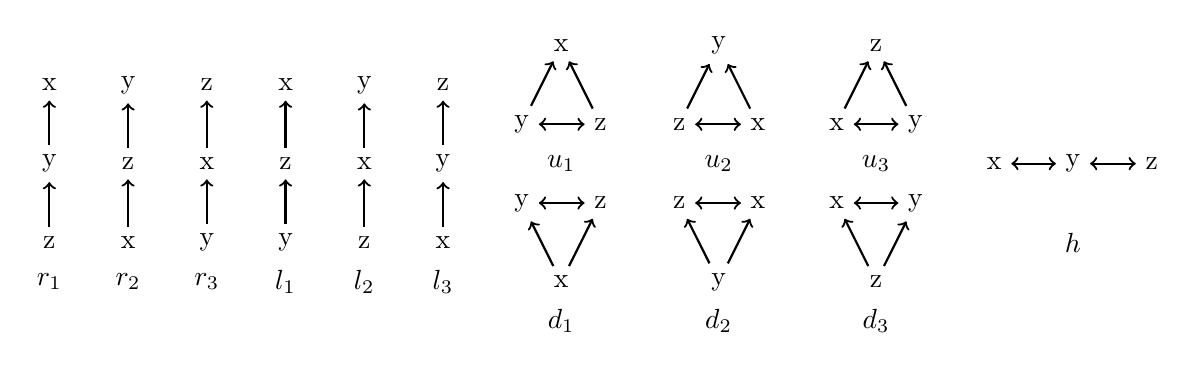
\begin{tikzpicture}
        \node (r1x) at (0,2) {x};  \node (r1y) at (0,1) {y};  \node (r1z) at (0,0) {z};  \node (r1n) at (0,-0.5) {$r_1$};
        \node (r2x) at (1,0) {x};  \node (r2y) at (1,2) {y};  \node (r2z) at (1,1) {z};  \node (r2n) at (1,-0.5) {$r_2$}; 
        \node (r3x) at (2,1) {x};  \node (r3y) at (2,0) {y};  \node (r3z) at (2,2) {z};  \node (r3n) at (2,-0.5) {$r_3$};
        \node (l1x) at (3,2) {x};  \node (l1y) at (3,0) {y};  \node (l1z) at (3,1) {z};  \node (l1n) at (3,-0.5) {$l_1$};
        \node (l2x) at (4,1) {x};  \node (l2y) at (4,2) {y};  \node (l2z) at (4,0) {z};  \node (l2n) at (4,-0.5) {$l_2$};
        \node (l3x) at (5,0) {x};  \node (l3y) at (5,1) {y};  \node (l3z) at (5,2) {z};  \node (l3n) at (5,-0.5) {$l_3$};
        \node (u1x) at (6.5, 2.5) {x};  \node (u1y) at (6.0, 1.5) {y};  \node (u1z) at (7.0, 1.5) {z};  \node (u1n) at (6.5, 1) {$u_1$};
        \node (u2x) at (9.0, 1.5) {x};  \node (u2y) at (8.5, 2.5) {y};  \node (u2z) at (8.0, 1.5) {z};  \node (u2n) at (8.5, 1) {$u_2$};
        \node (u3x) at (10.0,1.5) {x};  \node (u3y) at (11.0,1.5) {y};  \node (u3z) at (10.5,2.5) {z};  \node (u3n) at (10.5,1) {$u_3$};
        \node (d1x) at (6.5,-0.5) {x};  \node (d1y) at (6.0, 0.5) {y};  \node (d1z) at (7.0, 0.5) {z};  \node (d1n) at (6.5, -1) {$d_1$};
        \node (d2x) at (9.0, 0.5) {x};  \node (d2y) at (8.5,-0.5) {y};  \node (d2z) at (8.0, 0.5) {z};  \node (d2n) at (8.5, -1) {$d_2$};
        \node (d3x) at (10.0,0.5) {x};  \node (d3y) at (11.0,0.5) {y};  \node (d3z) at (10.5,-0.5){z};  \node (d3n) at (10.5,-1) {$d_3$};
        \node (hx) at (12,1) {x};  \node (hy) at (13,1) {y};  \node (hz) at (14,1) {z};  \node (hn) at (13,0.0) {$h$};
        \draw [thick,->] (r1z) -- (r1y); \draw [thick,->] (r1y) -- (r1x);
        \draw [thick,->] (r2x) -- (r2z); \draw [thick,->] (r2z) -- (r2y);
        \draw [thick,->] (r3y) -- (r3x); \draw [thick,->] (r3x) -- (r3z);
        \draw [thick,->] (l1y) -- (l1z); \draw [thick,->] (l1z) -- (l1x);
        \draw [thick,->] (l2z) -- (l2x); \draw [thick,->] (l2x) -- (l2y);
        \draw [thick,->] (l3x) -- (l3y); \draw [thick,->] (l3y) -- (l3z);
        \draw [thick,->] (u1y) -- (u1x); \draw [thick,->] (u1z) -- (u1x); \draw [thick,<->] (u1y) -- (u1z);
        \draw [thick,->] (u2z) -- (u2y); \draw [thick,->] (u2x) -- (u2y); \draw [thick,<->] (u2z) -- (u2x);
        \draw [thick,->] (u3x) -- (u3z); \draw [thick,->] (u3y) -- (u3z); \draw [thick,<->] (u3x) -- (u3y);
        \draw [thick,<-] (d1y) -- (d1x); \draw [thick,<-] (d1z) -- (d1x); \draw [thick,<->] (d1y) -- (d1z);
        \draw [thick,<-] (d2z) -- (d2y); \draw [thick,<-] (d2x) -- (d2y); \draw [thick,<->] (d2z) -- (d2x);
        \draw [thick,<-] (d3x) -- (d3z); \draw [thick,<-] (d3y) -- (d3z); \draw [thick,<->] (d3x) -- (d3y);
        \draw [thick,<->] (hx) -- (hy); \draw [thick,<->] (hy) -- (hz);
    \end{tikzpicture}
    \caption{3選択肢の選好}
\end{figure}

二分選好の集合DPの要素である選好の集合は,同率の選択肢が存在する選好のみからなるので,$DP = 2^{\{u_1,u_2,u_3,d_1,d_2,d_3,h\}} - \{\varnothing\}$です.

同調選好の集合EPでは,r,lが0個の要素は$\{u_1,u_2,u_3,d_1,d_2,d_3,h\}$の部分集合全体になります.r,lが1つある場合は以下,
\begin{equation*}
    \begin{array}[h]{c}
        \{r_1,u_1,u_2,d_2,d_3,h\},
        \{r_2,u_2,u_3,d_1,d_3,h\},
        \{r_3,u_1,u_3,d_1,d_2,h\},\\
        \{l_1,u_1,u_3,d_2,d_3,h\},
        \{l_2,u_1,u_2,d_1,d_3,h\},
        \{l_3,u_2,u_3,d_1,d_2,h\}
    \end{array}
\end{equation*}
の6つの各集合の部分集合全体になります.この表記だと$r_1$などr,lを含まない部分集合も含まれますが,そのような集合はr,lが0個の要素としてすでに検出したものと一致するので問題ありません.r,lが2つある場合は,
\begin{equation*}
    \begin{array}[h]{c}
        \{r_1,l_1,u_1,d_2,d_3,h\},
        \{r_1,l_2,u_1,u_2,d_3,h\},
        \{r_2,l_2,d_1,u_2,d_3,h\},\\
        \{r_2,l_3,d_1,u_2,u_3,h\},
        \{r_3,l_1,u_1,d_2,u_3,h\},
        \{r_3,l_3,d_1,d_2,u_3,h\}
    \end{array}
\end{equation*}
の6つの各集合の部分集合全体です.よって$EP$は,
\begin{align*}
EP = & 2^{\{u_1,u_2,u_3,d_1,d_2,d_3,h\}}\\
     & \cup 2^{\{r_1,u_1,u_2,d_2,d_3,h\}}
       \cup 2^{\{r_2,u_2,u_3,d_1,d_3,h\}}
       \cup 2^{\{r_3,u_1,u_3,d_1,d_2,h\}}\\
     & \cup 2^{\{l_1,u_1,u_3,d_2,d_3,h\}}
       \cup 2^{\{l_2,u_1,u_2,d_1,d_3,h\}}
       \cup 2^{\{l_3,u_2,u_3,d_1,d_2,h\}}\\
     & \cup 2^{\{r_1,l_1,u_1,d_2,d_3,h\}}
       \cup 2^{\{r_1,l_2,u_1,u_2,d_3,h\}}
       \cup 2^{\{r_2,l_2,d_1,u_2,d_3,h\}}\\
     & \cup 2^{\{r_2,l_3,d_1,u_2,u_3,h\}}
       \cup 2^{\{r_3,l_1,u_1,d_2,u_3,h\}}
       \cup 2^{\{r_3,l_3,d_1,d_2,u_3,h\}}
       - \{\varnothing\}
\end{align*}
です.

敵対選好の集合$AP$は,r,lが0の要素は先程と同様に$\{u_1,u_2,u_3,d_1,d_2,d_3,h\}$の部分集合全体です.r,lが3つ以上含まれることはありません.r,lが1つまたは2つある時は,
\begin{equation*}
    \{r_1,l_3,u_2,d_2,h\},\{r_2,l_1,u_3,d_3,h\},\{r_3,l_2,u_1,d_1,h\}
\end{equation*}
の各集合の部分集合全体です.よって,$AP$は,
\begin{align*}
AP = & 2^{\{u_1,u_2,u_3,d_1,d_2,d_3,h\}} 
       \cup 2^{\{r_1,l_3,u_2,d_2,h\}} \\
     & \cup 2^{\{r_2,l_1,u_3,d_3,h\}} 
       \cup 2^{\{r_3,l_2,u_1,d_1,h\}}
       - \{\varnothing\}
\end{align*}
です.

極値制限の集合$ER$は,r,lが0,1つの時は$EP$と同じになります.r,lが3つ以上含まれることはありません.r,lが2つのときは
\begin{equation*}
    \begin{array}[h]{c}
        \{r_1,l_1,u_1,d_2,d_3,h\},
        \{r_1,l_2,u_1,u_2,d_3,h\},
        \{r_1,l_3,d_2,u_2,h\},     \\
        \{r_2,l_1,u_3,d_3,h\},
        \{r_2,l_2,d_1,u_2,d_3,h\},
        \{r_2,l_3,d_1,u_2,u_3,h\}, \\
        \{r_3,l_1,u_1,d_2,u_3,h\}.
        \{r_3,l_2,d_1,u_2,u_3,h\},
        \{r_3,l_3,d_1,d_2,u_3,h\}
    \end{array}
\end{equation*}
です.よって$ER$は,
\begin{align*}
ER = & 2^{\{u_1,u_2,u_3,d_1,d_2,d_3,h\}}\\
     & \cup 2^{\{r_1,u_1,u_2,d_2,d_3,h\}}
       \cup 2^{\{r_2,u_2,u_3,d_1,d_3,h\}}
       \cup 2^{\{r_3,u_1,u_3,d_1,d_2,h\}}\\
     & \cup 2^{\{l_1,u_1,u_3,d_2,d_3,h\}}
       \cup 2^{\{l_2,u_1,u_2,d_1,d_3,h\}}
       \cup 2^{\{l_3,u_2,u_3,d_1,d_2,h\}}\\
     & \cup 2^{\{r_1,l_1,u_1,d_2,d_3,h\}}
       \cup 2^{\{r_1,l_2,u_1,u_2,d_3,h\}}
       \cup 2^{\{r_1,l_3,u_2,d_2,h\}}    \\
     & \cup 2^{\{r_2,l_1,u_3,d_3,h\}}
       \cup 2^{\{r_2,l_2,d_1,u_2,d_3,h\}}
       \cup 2^{\{r_2,l_3,d_1,u_2,u_3,h\}}\\
     & \cup 2^{\{r_3,l_1,u_1,d_2,u_3,h\}}
       \cup 2^{\{r_3,l_2,u_1,d_1,h\}}
       \cup 2^{\{r_3,l_3,d_1,d_2,u_3,h\}}
       - \{\varnothing\}
\end{align*}
です.以上より,$DP \cup AP \cup EP$を計算すると$ER$と同じになり,$DP \cup AP \cup EP = ER$です.よって二分選好,敵対選好,同調選好のどれかであることは価値制限を満たすことと同値です.
\end{proof}

図13について考えます.$DP \subset AP$,$DP \subset EP$となることは簡単に確認できます.$|DP|$は,
\begin{equation*}
    |DP| = 2^7 - 1 = 127
\end{equation*}
です.

$AP \cap EP$は,
\begin{align*}
    AP \cap EP = &
        2^{\{u_1,u_2,u_3,d_1,d_2,d_3,h\}} \\
      & \cup 2^{\{r_1,u_2,d_2,h\}} 
        \cup 2^{\{r_2,u_3,d_3,h\}} 
        \cup 2^{\{r_3,u_1,d_1,h\}} \\ 
      & \cup 2^{\{l_1,u_3,d_3,h\}} 
        \cup 2^{\{l_2,u_1,d_1,h\}} 
        \cup 2^{\{l_3,u_2,d_2,h\}} - \{\varnothing\}
\end{align*}
ですが,重複部分がないようにすると,
\begin{align*}
    AP \cap EP = &
        2^{\{u_1,u_2,u_3,d_1,d_2,d_3,h\}} \\
      & \cup (2^{\{r_1,u_2,d_2,h\}} - 2^{\{u_2,d_2,h\}})
        \cup (2^{\{r_2,u_3,d_3,h\}} - 2^{\{u_3,d_3,h\}}) \\
      & \cup (2^{\{r_3,u_1,d_1,h\}} - 2^{\{u_1,d_1,h\}})  
        \cup (2^{\{l_1,u_3,d_3,h\}} - 2^{\{u_3,d_3,h\}}) \\
      & \cup (2^{\{l_2,u_1,d_1,h\}} - 2^{\{u_1,d_1,h\}}) 
        \cup (2^{\{l_3,u_2,d_2,h\}} - 2^{\{u_2,d_2,h\}}) - \{\varnothing\}
\end{align*}
であり,結局,
\begin{equation*}
    |AP \cap EP| = 2^7 + 6 \times (2^4 - 2^3) - 1 = 175 
\end{equation*}
です.同様にして,
\begin{equation*}
    |AP| = 2^7 + 3 \times (2^5 - 2^3) - 1 = 199
\end{equation*}
\begin{equation*}
    |EP| = 2^7 + 6 \times (2^6 - 2^5) + 6 \times (2^6 - 2^5 - 2^5 + 2^4) - 1 = 415
\end{equation*}
となり,図13が書けます.

さて,多数決決定法がどのような時にアロー4条件を見てきたのですが,図13を見ると3選択肢で極値制限を満たす,すなわちその制限の中では個人的選好の自由が保証されるというような選好の組は全体の5\%程度しかありません.

参考文献[3]によると,同率を許さない強順序の選好を各個人がランダムに行った時,3選択肢での多数決決定法で勝者,すなわち,他のどの選択肢に対しても多数となっているような選択肢が現れない確率は図14のようになります.

\begin{figure}[!h]
    \centering
    \begin{tabular}{|cc|cc|} \hline
        人数 & 確率 & 人数 & 確率 \\ \hline 
         1 & 0.0000 & 17 & 0.0827 \\ 
         3 & 0.0556 & 19 & 0.0832 \\ 
         5 & 0.0694 & 21 & 0.0836 \\ 
         7 & 0.0750 & 23 & 0.0840 \\ 
         9 & 0.0780 & 25 & 0.0843 \\ 
        11 & 0.0798 & $\vdots$ & $\vdots$ \\
        13 & 0.0811 & $\infty$ & 0.0877 \\ 
        15 & 0.0820 & & \\ \hline
    \end{tabular}
    \caption{3選択肢で多数決決定法の勝者が現れない確率}
\end{figure}

こうして見ると,3選択肢に限れば,たとえどれだけの人がいても9割以上の確率で決着が付くのです.次に人数を無限にしたままで選択肢の数を増やして行ったものが図15です.

\begin{figure}[!h]
    \centering
    \begin{tabular}{|cc|cc|} \hline
        選択肢 & 確率   & 選択肢 & 確率 \\ \hline
        1      & 0.0000 & 20     & 0.6811 \\
        2      & 0.0000 & 25     & 0.7297 \\
        3      & 0.0877 & 30     & 0.7648 \\
        4      & 0.1755 & 35     & 0.7914 \\
        5      & 0.2513 & 40     & 0.8123 \\
        10     & 0.4887 & 45     & 0.8292 \\
        15     & 0.6087 & & \\ \hline
    \end{tabular}
    \caption{n選択肢で多数決決定法の勝者が現れない確率}
\end{figure}

今度はかなり急激に確率が上昇してしまいます.選択肢が10を超えると半分以上の確率で勝者が決まりません.20にもなると,7割近くで決着が付きません.極値制限を満たしていれば決着はつきますが,決着が付くからと言って極値制限を満たしているわけではないですし,こう見ると極値制限を満たしているという条件はずいぶん個人的選好を制限してしまっているというふうに捉えても良いように思えます.

しかし,極値制限の導入を完全に否定しきることも難しいです.今まで多数決決定法がアロー4条件を満たすための個人的選好の制限について見てきましたが,これは社会の構成員が皆互いにある程度類似した判断をしている時は社会的な決定に決着が付くということだと考えても良いでしょう.こうなると,ある程度の制約を満たしていることが社会で合意を得るために必要な条件だということで,個人が相互配慮をして選好することを社会的な規則として導入するということも,民主的な投票と言える範疇から外れないのではないかというようにも考えられないでしょうか.

我々人間も所詮は動物なのです.我々の社会を個体の集団として捉えると,その社会の維持のために動物的本能として軋轢を生じさせないように意見を変えさせるような社会的圧力を受け入れるというのは,一見民主的ではないように思えても,生態系という観点から見ると自然なことだと言うこともできるでしょう.

しかし,そもそもこの極値制限に道徳的解釈や倫理的正当化を付すことができるでしょうか?もし,それができるような文化であれば,そのような投票方式が採用されるのかもしれませんが,実際には,「運良くこういうパターンの選好になったら,多数決決定法でも循環が起きたりしない」以上の意味合いを持たせられないようにも思えます.

多数決決定法を正当化するには,この個人的選好の自由という条件についてだけ見るのでは苦しいような気もします.他の条件についても考えてみましょう.


